\documentclass[11pt]{article}
\usepackage[utf8]{inputenc}
\usepackage{graphicx}
\usepackage{url}
\usepackage{amsmath}
\usepackage{float}


\title{
	{Computer Vision 1 - Assignment 2 \\
	Linear Filters: Gaussians and Derivatives}
}
\author{
Selene Baez Santamaria (10985417) - Andrea Jemmett (11162929)}
\date{\today}

\begin{document}

\maketitle


\section{1D Gaussian Filter}
% Question: "Compare your function with MATLAB’s built-in fspecial. What are the differences?"
Our function takes the same arguments as the built-in fspecial, but it generates different output. On the one hand our function generates a vector of size $kernelLength$. On the other hand, the fspecial function returns a rectangular or squared matrix dependant on the hsize parameter. 


\section{Convolving an image with a 2D Gaussian}
% Question 1:
% Show that the outputs of convolution with the 2D kernel (i.e. the one corresponding to the two 1D kernels) and convolution with 1D kernels are essentially the same.
% Use kernel length of 11.
% Report the numerical equivalence as well as plots at every stage of filtering pipeline.
% Question 2: Explain the benefits of kernel separability, shortly.
We use a value of $\sigma_x = 2$ and $\sigma_y = 2$ and a kernel length of 11. First we call the gaussian function defined in the prefious section to get two 1D filters, one with each $\sigma$. We multiply this 1D vector by its traspose to get a 2D gaussian filter. 

To convolve the images and filters we use the built-it function $conv2$. After testing the different options we found out the following:

\begin{itemize}
	\item "full": performs the full convolution. Visually, we note that the produced images have black frames on the edges since the dimensions are slightly (10 pixels) larger than the original image.
	\item "valid": performs convolution but omits padding %TODO
	\item "same": performs the convolution and returns an image that is the same size as the filter. 
\end{itemize}

In order to check that both functions produce the same images we make a pixel per pixel comparison. We check that the absolute value of the difference among the values is less that a small value $\epsilon = 1 e^12$. Hereby we show the original and filtered images using the "full" option:

\begin{figure}[H]
	\centering
	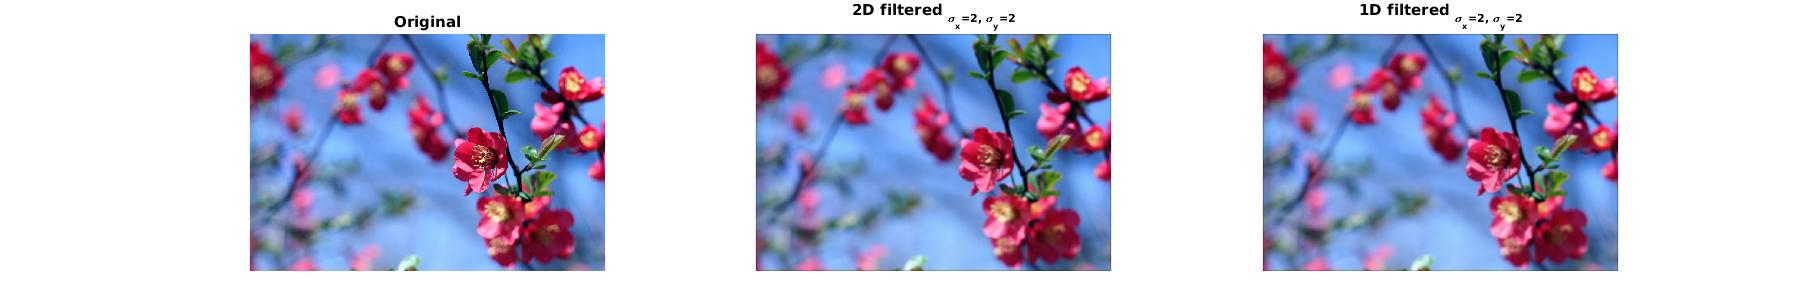
\includegraphics[width=.9\textwidth]{imgs/flowers_conv.jpg}
	\caption{Comparison for flowers.jpg.}
	\label{fig:flowers}
\end{figure}

\begin{figure}[H]
	\centering
	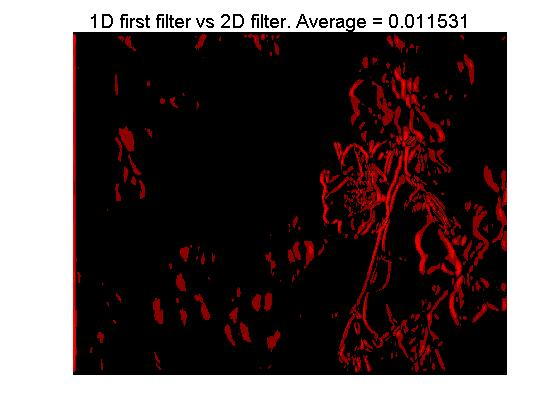
\includegraphics[width=.9\textwidth]{imgs/flowers_col_heatmap.jpg}
	\caption{Heatmap showing the absolute difference per pixel between Step 1 of 1D filtering and 2D final filtered image for flowers.jpg. Reported mean error per pixel is $0.0115$}
	\label{fig:flowers_col_heatmap}
\end{figure}

\begin{figure}[H]
	\centering
	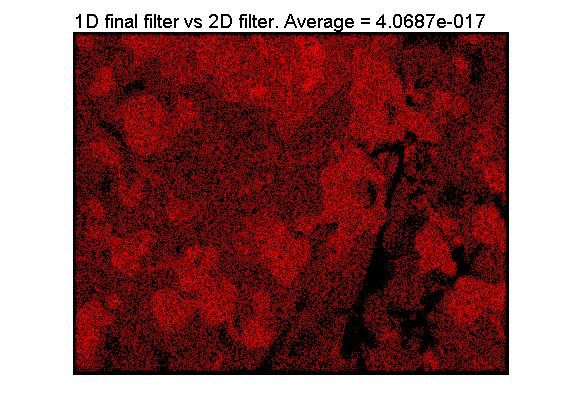
\includegraphics[width=.9\textwidth]{imgs/flowers_heatmap.jpg}
	\caption{Heatmap showing the absolute difference per pixel between both final filtered images for flowers.jpg. Reported mean error per pixel is $4.0687 e^-017$}
	\label{fig:flowers_heatmap}
\end{figure}

\begin{figure}[H]
	\centering
	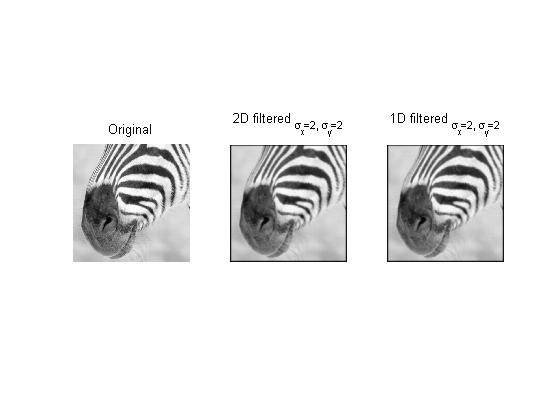
\includegraphics[width=.9\textwidth]{imgs/zebra_conv.jpg}
	\caption{Comparison for zebra.png. Reported mean error per pixel is $5.5609 e^-017$}
	\label{fig:zebra}
\end{figure}

\begin{figure}[H]
	\centering
	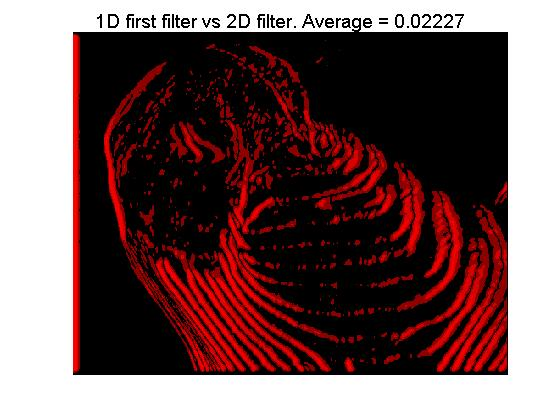
\includegraphics[width=.9\textwidth]{imgs/zebra_col_heatmap.jpg}
	\caption{Heatmap showing the absolute difference per pixel between Step 1 of 1D filtering and 2D final filtered image for zebra.png. Reported mean error per pixel is $0.0223$}
	\label{fig:zebra_col_heatmap}
\end{figure}

\begin{figure}[H]
	\centering
	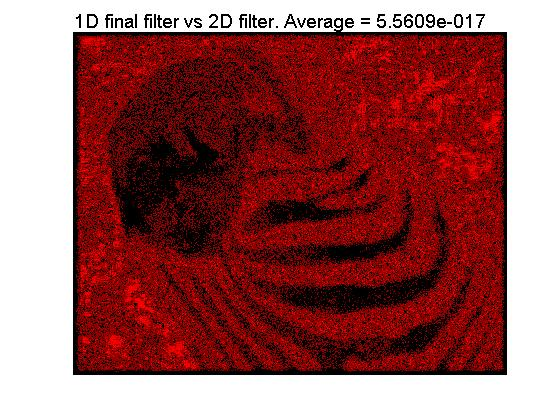
\includegraphics[width=.9\textwidth]{imgs/zebra_heatmap.jpg}
	\caption{Heatmap showing the absolute difference per pixel between both final filtered images for zebra.png. Reported mean error per pixel is $5.5609 e^-017$}
	\label{fig:zebra_heatmap}
\end{figure}

%We note that the 1D convoluted image takes longer to compute. 
Having kernel separability is helpful since the computation time is reduced. 

\section{Gaussian Derivative}


The Gaussian derivative may be used to find edges in am image. An application could be countoruing an image.

\end{document}

